\usepackage{enumitem}
\chapter*{Project 2: The Circle of Life - Create a Board Game}
\addcontentsline{toc}{chapter}{Project 2: The Circle of Life}
\setcounter{chapter}{8}
\setcounter{section}{0}

\begin{abstract}
This project will get you familiar with:
\begin{enumerate}
    \item Objects
    \begin{itemize}
        \item Designing objects and complete member function lists
        \item Making objects that store other objects
    \end{itemize}
    \item User interface design
\end{enumerate}

\textbf{Warning:} You are not allowed to use global variables, pointers, or pass-by references for this assignment.

\end{abstract}

\begin{figure}[h!]
    \centering
    
\includegraphics[width=0.75\linewidth]{images/Savanna.jpg}
\end{figure}

%TO-DO: for spring: make Tile just a struct, suggest the Game class for a 3rd class instead.

\section{\textbf{Introduction}}

For the Final Project, you will implement a text-based, 2-player board game in C++ that draws inspiration from Disney's \textit{The Lion King}. 

Players will journey across the African Savannah, each as a young lion eager to prove they're ready to step up as the next `Pride Leader' after Simba's retirement. Along the way, they'll make strategic decisions, face unexpected challenges, and collect Pride Points as they grow and refine their Leadership Traits—Stamina, Strength, and Wisdom. Whether navigating tricky terrain or helping a fellow lion in need, each choice will shape their journey. The player who earns the most Pride Points by demonstrating they have what it takes to guide the pride's future will be chosen as the next `Pride Leader', ensuring the pride is thriving and keeping the circle of life moving forward! 

Unlike previous assignments, this project has no answer key, prebuilt test cases, or set questions. Instead, you'll be given a list of requirements to meet, and it's up to you to fulfill them in the most creative way possible. 

This project will be worth more of your grade than any previous assignment. We recommend starting early to give yourself enough time to complete it. This is worth 10\% of your final grade. 

\section{\textbf{Game Play}}

The goal of this game is simple: as a player, you'll lead your lion on one of two distinct paths—either through Cub Training or Straight to the Pride Lands. Each path offers its own unique set of advantages and challenges, shaping your journey and influencing your growth along the way. As you advance, you'll cross different terrain: grasslands, drylands, wetlands, and unknown terrain, which introduce unexpected obstacles that may either help or hinder your progress. Navigate these challenges wisely to prove that you have what it takes to become the next `Pride Leader.' 

We have outlined the critical components of the game below, but there are numerous opportunities for creative expression in how you choose to define the details of your game. There is no CodeRunner that you have to match precisely, so take advantage of the flexibility here. Whenever we do not explicitly provide details on a given mechanic in the game, please use your own intuition to design an interesting and cohesive game.


\subsection{Starting the Game}
This is a two-player game. First, display all available characters and their stats. Then, prompt the players to enter their names and select a lion character. Both players choose a character from the predefined list of five character lions (see character.txt), with each featuring various personal attributes such as name and age (see Character Selection Menu). After selecting a character and before the first turn, players also choose their Path Type, which is either Cub Training or Straight to the Pride Lands (see Path Types). Each path type will contain the same number of special tiles (unique events that affect Leadership Traits) and regular tiles (random events that affect Pride Points). However, the arrangement of the tiles will differ depending on the path chosen (See Visual Board Representation). %I'm still not clear on why this should be a struct?? What are they actually supposed to store?

For each turn in the game, you should display the Main Menu, including the current position of players on the board and a relevant Main Menu for the space the player is currently on (see Main Menu in Feature Requirements).

\subsection{Character Selection Menu}
The \verb|characters.txt| file contains a list of playable lions that players can choose from(See the example of the character file below). Each lion entry includes the following attributes: Name, Age, Strength, Stamina, Wisdom, and Pride Point. When players select a character, they will start the game with the predetermined point value for Leadership Traits and Pride Point associated with that character (see example ranges below). Ensure that each character can only be chosen once, and update the menu to show only the available characters. 

Example of \verb|characters.txt|:
\begin{verbatim}
playerName|age|strength|stamina|wisdom|pridePoints
Apollo|5|500|500|1000|20000
Mane|8|900|600|600|20000
Elsa|12|900|700|500|20000
Zuri|7|600|500|900|20000
Roary|18|1000|500|500|20000
\end{verbatim}

Each player begins with 20,000 Pride Points before choosing their Path Type. The starting number of Leadership Traits varies for each character. The Path Type chosen can increase or decrease the number of Leadership Traits and Pride Points from the characters' starting values. It's important to note that the values for Stamina, Strength, and Wisdom cannot go below 100 Points throughout the entire game. If the values are below 100, default them to 100. % To do this, you will create a condition that specifies ``anytime that either of the Leadership Traits go below 100 Points, default to 100 Points as this is the minimum Points for each Leadership Trait."


\subsection{Path Types}
During game setup, ask each player to choose one of two path types. These path types will impact the starting stats for the player as well as the arrangement of the tiles they will follow on the game board. More details on how each path will impact the game board are available in section 3.2 (Visual Board Representation). 

The two path options are listed below:

\subsubsection{Cub Training:} 

This path equips your lion character with essential Leadership Traits—Stamina, Strength, and Wisdom—needed for future leadership. The training requires an investment of -5,000 Pride Points from the starting number of Pride Points; this symbolizes the time and resources dedicated to developing these skills instead of gaining Pride Points. This path also adds 500 Stamina Points, 500 Strength Points, and 1,000 Wisdom Points to the starting amount of your character's Leadership Traits before you start the journey. Choosing this path allows your character to grow and mature, gaining valuable abilities at the expense of early progress. Although this path slows down your initial Pride Point accumulation, the boost in key traits and the opportunity to select an advisor for mentorship prepare your character for greater challenges and future leadership potential. 
\begin{itemize}
    \item Advisor Choice: If the player selects Cub Training, they will be prompted to choose an advisor who grants a unique special ability that protects them during random events that have a negative influence on their Pride Points (please see Advisor List).
\end{itemize}

\subsubsection{Straight to the Pride Lands:} This option lets your lion character jump directly into life on the Savannah with an immediate boost of +5,000 Pride Points from the starting number of Pride Points, allowing early progression and quick success in achieving intermediate goals. This path adds 200 Stamina Points, 200 Strength Points, and 200 Wisdom Points to the starting amount of your character's Leadership Traits before you start the journey, leaving your character with fewer resources to prepare for more difficult situations. Also, you do not get an initial Advisor if you choose this path. Although this path offers a strong head start, it lacks the long-term resilience and special abilities that could be gained through mentorship in Cub Training, making it a riskier approach to becoming a Pride Leader. 


\subsection{Advisor List}
The advisors have special abilities that can protect you in case of a negative random event (see the example below of the \verb|random_events.txt| file). You should choose your advisor wisely.
\begin{enumerate}

\item Rafiki - Invisibility (the ability to become un-seen)
\item Nala - Night Vision (the ability to see clearly in darkness)
\item Sarabi - Energy Manipulation (the ability to shape and control the properties of energy)
\item Zazu - Weather Control (the ability to influence and manipulate weather patterns)
\item Sarafina - Super Speed (the ability to run 4x faster than the maximum speed of lions)



\end{enumerate}


Example of \verb|random_events.txt|:
\begin{verbatim}

Description | PathType (0 = cubTraining; 1 = straight to the pride lands; 2 = either path) | 
Advisor (0 = none; 1 = Rafiki; 2 = Nala; 3 = Sarabi; 4 = Zazu; 5 = Sarafina) | PridePoints (lose or gain)

Desert storm sweeps through the territory|2|4|-500
Fatigue from intense training with pride warriors|0|3|-200
Challenging night watch duty under pitch-black conditions|1|2|-400
Extra energy from bountiful season|1|0|800
Observed a rare natural phenomenon|0|0|600
Gained wisdom from observing Rafiki’s rituals|1|0|500

\end{verbatim}

For example, players on either path could encounter ``Desert storm sweeps through the territory", but if you have Zazu as your advisor, you will safely bypass that event. If you do not have Zazu as advisor, you will suffer -500 pride points. 

However, only players that chose to do cub training would be able to encounter ``Fatigue from intense training with pride warriors". They would be safe if they had Sarabi as an advisor and skip the event, but if they had any other advisor, they would lose 200 pride points.

\subsection{Core Concepts of the Game}
\begin{enumerate}
    \item The game starts by selecting your preferred lion character from a list of available character names.
    \item Select a path type for your chosen Lion character from the two path types: Cub Training or Straight to the Pride Lands. Each of these paths differs in what they offer.
    \item The map is a two-lane path (one lane for each path type). Depending on the path type chosen, both players can be on the same path or on different paths (See Visual Board Representation for details). Players navigate by spinning a virtual spinner (players can land on any number from (1-6) to determine how far to move forward. You can do this by using a random number generator.
    \item Players alternate taking turns playing each round of the game.
    \item There are special tiles on the game board where unique events happen that can affect your Leadership Traits or other aspects of the game (please see Special Tiles section)
    \item The players must manage their total Stamina, Strength, Wisdom, and Pride Points throughout the game.
    \item If you did not choose the cub training path, advisor selection is available on some special tiles where players can select an advisor (see Counseling Tile under Special Tiles). Advisors have special abilities in the random event files, depending on the path type of the character that holds it. If a player already has an advisor, you cannot select that same advisor. 
    \item Negative events occasionally occur, causing players to lose Leadership Traits or Pride Points that can setback their journey to becoming the Pride Leader.
    \item Once all players reach Pride Rock, represented by the Orange Tile, the player who has the highest Pride Points wins the game.
\end{enumerate}
 

 
\section{\textbf{Feature Requirements}}

The minimum requirements for this final project are given in the following sections. You are not allowed to use pointers, global variables, or pass-by-reference in the project. 


\subsection{Interactive Components}
\begin{itemize}
            \item Players move forward on the board by spinning a virtual spinner, similar to the image shown below. The number of tiles they land on determines how many tiles they advance on their turn. You can do this by using a random number generator (you do not need to actually draw a spinner -- printing the random output is sufficient).
\begin{figure}[h!]
    \centering
    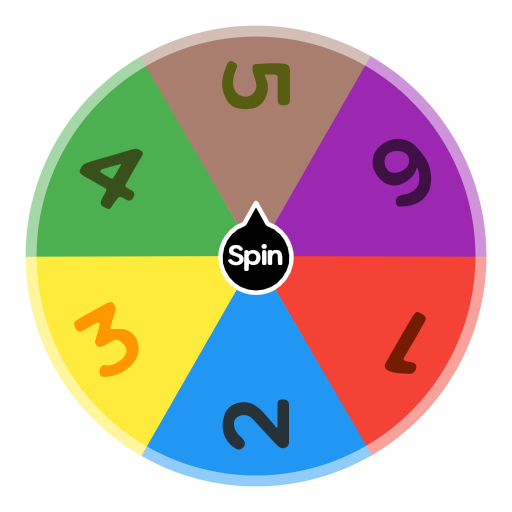
\includegraphics[width=0.5\linewidth]{images/spinner.png}
\end{figure}
            \item Design the two distinct starting paths for players to choose from—one path requires an initial investment for  \textit{greater resources} (such as less Pride Points but more Leadership Trait Points) that lead to long-term rewards, while the other provides an immediate reward with higher starting points but \textit{fewer resources} (such as more Pride Points but less Leadership Trait Points), impacting potential growth over time.  
            \item Respond to in-game events and challenges, such as choosing actions, providing answers, or otherwise reacting to encountered situations, which may include solving riddles or making strategic choices based on the scenario presented. 

\paragraph{Main Menu}
Provide an interactive menu with at least five options. For example, when players open the main menu, they may see the following options: 
\end{itemize}

\begin{enumerate}
    
\item Check Player Progress: Review Pride Point and Leadership Trait stats.
\item Review Character:  Check your character name and age. 
\item Check Position: Display board to view current position.
\item Review your Advisor: Check who your current advisor is on the game.
\item Move Forward: For each player's turn, access this option to spin the virtual spinner.
\end{enumerate}

    At least 2 of the options should have secondary layers. For example: 
        \begin{itemize}
        \item Review Your Advisor could have an additional option that displays the advisor’s ability and prompts the player to confirm using it.
        \item Check Player Progress has an additional option to convert Leadership Traits to Pride Points (see winning the game details on the purpose of converting Leadership Traits to Pride Points).
        \end{itemize}

Example of the Main Menu:
\begin{verbatim}
Main Menu: Select an option to continue 
1. Check Player Progress (1)
2. Review Character (2)
3. Check Position (3)
4. Review your Advisor (4)
5. Move Forward (5)

Please choose an option using the corresponding number: 
\end{verbatim}

\subsection{Visual Board Representation}
\subsubsection{\textbf{Step 1. Set Up the Initial Board Structure}}
\begin{itemize}
    \item Use the provided board files, \verb|board.cpp| and \verb|board.h|, to display the 52-tile trail on a 2-lane path (one lane for each path type, with a total of 104 tiles) (see Figure 1). 
    \item Ensure that the Starting Tile (Gray Color) and Ending Tile(Orange Tile) are visible on both lane paths. You may want to label which path corresponds to Cub Training, and which path corresponds to Straight to the Pride Lands.
    \item Ensure that the board contains a minimum of 102 tiles in various colors (e.g., Pink, Green, Blue) to represent different tile types.
    \item \textbf{Randomize the tile arrangement}: The tiles on the map should be randomized each time the game starts. Additionally, ensure that the distribution rules for the tiles differ between the two paths (Cub Training and Straight to the Pride Lands), creating unique gameplay experiences for each path. You should design your own rules for the tile generation based on what you think makes sense and would create a well-balanced game. Should players who have advisors and went through Cub Training have fewer challenges right away, while those who went straight to the pride lands are more likely to struggle early on? You must \textbf{randomize each path}, and the distribution rules for each path \textbf{must be different}.
    \item The provided example board currently displays starting tile, regular tile, special tile, and ending tile templates. You need to implement the functioning of each of these tile types on the board. For each lane, ensure there are at least 20 special tiles with unique characteristics spread randomly across the board. Each tile should have a distinct purpose; examples are detailed below in the ``Tile Details/Descriptions" subsection.
    \item The Final Tile is named ``Pride Rock." This tile signifies the game's endpoint and should convert the Leadership traits to Pride Points to determine and congratulate the winner!
\end{itemize}

\begin{figure}[h!]
    \centering
    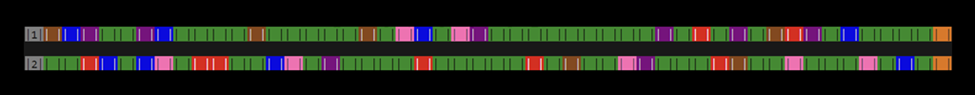
\includegraphics[width=1\linewidth]{images/BoardExample.png}
    \caption{Example of the 2-lane Board when players choose \textbf{different path types}}
\end{figure}
\begin{figure}[h!]
    \centering
    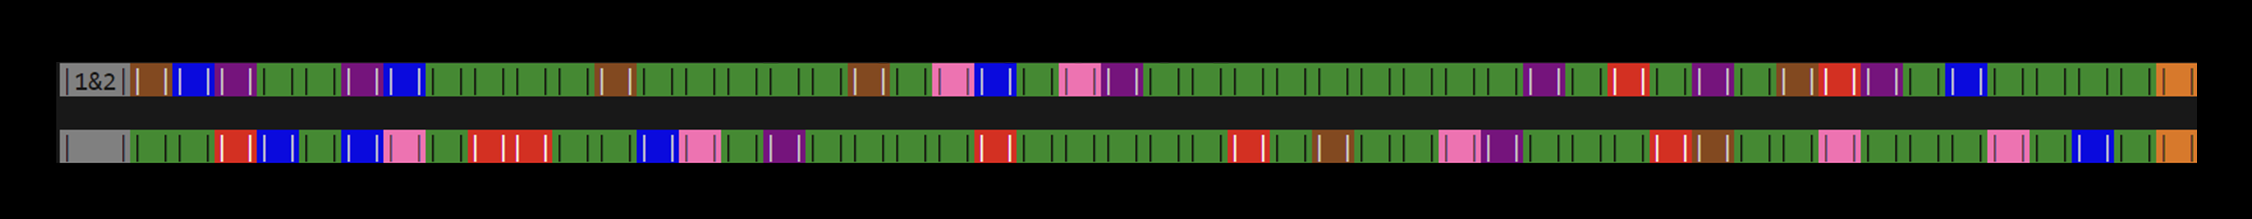
\includegraphics[width=1\linewidth]{BoardExample2.png}
    \caption{Example of the 2-lane Board when players choose \textbf{the same path type}}
\end{figure}
\subsubsection{\textbf{Step 2. Implement Player Representation on the Board}}
Add functionality to visually represent each player's position on the board using numbers:
\begin{itemize}
    \item Use ``1" to represent Player 1 and ``2" to represent Player 2.
    \item The Final Tile is colored orange, and it represents Pride Rock.
    \item The Starting Tile is colored gray, and it represents the Starting Point after both players have decided on their path choices.
    \item Update each player's position on the board and display the board at the end of every turn. The position should reflect any forward or backward moves resulting from the game spinner or event outcomes.
\end{itemize}


\subsection{Tile Details/Descriptions}
\textbf{Regular Tiles:} These tiles represent random events that have probability-based outcomes.
    \begin{itemize}
        \item Regular tiles are colored green to represent the grassy lands of the Savannah; anything can happen in this open landscape. For each path, ensure there is a minimum of 20 regular tiles on the board. When triggered, randomly select an event from the \verb|random.txt| file's event list that impacts the player's Pride Points either positively or negatively. Implement a 50\% chance for an event to be triggered when landing on these regular tiles. The random events are dependent on the path type. In addition, the current player's advisor protects against random events that have a negative influence on Pride Points.
    \end{itemize}
    
\textbf{Special Tiles:} These tiles are full of surprises, adding twists and turns to your journey. There should be at least 20 special tiles with random positions across each lane of the board. When triggered, events from the special tiles impact the player's current positions,  Leadership Traits (Stamina, Strength, and Wisdom), or other attributes. The special tiles are listed below: 
    \begin{itemize}
        \item Oasis Tile (blue color tile): You've found a peaceful oasis! This grants the player an extra turn to keep moving forward—take a deep breath and relax; you also gain 200 Stamina, Strength, and Wisdom Points.
        \item Counseling Tile (pink color tile): Welcome to the land of enrichment - when landing on this tile, your Stamina, Strength, and Wisdom Points increase by 300, and you get to choose an advisor from the available list of advisors. If you already have an advisor, you can switch your advisor out for a different one from the list or keep your original advisor. Don't forget - an advisor can protect you from random events that negatively impact your Pride Points.
        \item Graveyard Tile (red color tile): Uh-oh, you've stumbled into the Graveyard! This forces the player to move back 10 tiles and lose 100 Stamina, Strength, and Wisdom Points.
        \item Hyenas Tile (brown color tile): The Hyenas are on the prowl! They drag you back to where you were last, and the journey comes at a cost. This returns the player to their previous position. In addition, the player's Stamina Points decrease by 300 Points.
        \item Challenge Tile (purple color tile): Time for a test of wits! Land here, and you'll face a riddle randomly pulled from the \verb|riddles.txt| file.  Answer correctly, and you'll earn a boost of 500 Points to your Wisdom Trait—your cleverness pays off!
    \end{itemize}

Example of the \verb|riddles.txt| file:
\begin{verbatim}
Question(answer specifications)|Answer
I can hold multiple functions, but I’m not a list. What am I? (single word, lowercase)|class
I start a comment in C++. What am I? (symbol)|//
I am the number of bits in a byte. What am I? (integer)|8


\end{verbatim}

\section{\textbf{Implementation Requirements}}

\subsection{Class Structures:}
These classes are strongly encouraged, but this is not an exhaustive list of classes that may be valuable in your code. 
\begin{itemize}

    \item \mintinline{c++}{Board} Class: Represents the game board with an array or vector of \mintinline{c++}{Tile} objects, each with specific properties and types.
    \item \mintinline{c++}{Tile} Class: Represents each tile, with attributes for type (e.g., Green, Pink, Blue) and references to any potential effects (e.g., challenges, random events). This could also be a struct.
    \item     \mintinline{c++}{Player} Class: Tracks player attributes, including Pride Points, Stamina, Strength, and Wisdom. Includes methods for adjusting these attributes based on events.

\end{itemize}


\subsection{Data Members and Methods:}
\begin{itemize}
    \item Ensure each required class has at least 4 data members, with appropriate getters, setters, and constructors.
    \item Use an array or vector of objects from one user-defined class within another (e.g., an array of Tile objects within the \mintinline{c++}{BoardClass}).
\end{itemize}


\subsection{File I/O:}
\begin{itemize}
    \item Write game stats to a file at the end of the game.
    \item Read files such as \verb|random_events.txt|, \verb|riddles.txt|, and \verb|characters.txt|
\end{itemize}


\subsection{Code Structure and Flow Control:}
Include the following:
\begin{itemize}
    \item 6+ if-else statements for game events, advisor choice, and board tile actions.
    \item 6+ loops, including at least 2 nested loops, to manage board traversal, player turns, and challenge encounters.
\end{itemize}


\subsection{Final Evaluation:}
\begin{itemize}
    \item \textbf{All players reach final tile}: Calculate each player's total Pride Points. For every 100 points in Stamina, Strength, or Wisdom, add 1,000 Pride Points to their Pride Points total. 
    \item \textbf{Declare the winner}: Display the name of the lion with the highest Pride Points as the winner, along with each player’s final stats. 
\end{itemize}

Note: For any requirements not explicitly detailed, use your own creativity to design an interesting and cohesive gameplay experience. 

\section{\textbf{Group Work Overview}}

You are allowed to work with (at most) one other student who is currently in CSCI 1300 this semester (in any section). You may also work by yourself if you choose.

If you choose to work in a group, there are additional requirements. We expect that you will contribute equally to the project. Both group members must submit a zip file for the project, and the solution files can be the same. Indicate your partner’s name in the comments at the top of each code file.


\subsection{Group Requirements}
In addition to the requirements reviewed above, if you work in a group, you must also implement a sorting algorithm and apply it to a task in your program, and at least one other customization in your code. You should not use a Library function or any external resources to implement the sorting algorithm. Possible customizations are listed below.

One situation where the sorting functionality would be useful is for a ranking task, for example, ranking all the players who have completed this game based on their final pride point values. 

Note:
\begin{itemize}
    \item If you work in a team and you do not implement a sorting task, 50 points will be deducted from your point total.
    \item We expect that you will be contributing to the project equally. Both group members must submit a zip file for the project, and the solution files can be the same. Indicate your partner’s name in the comments at the top of each code file. Both partners will book an interview grading appointment together, and TAs will grade you individually.
\end{itemize}



\section{\textbf{Customization}}

This game is inspired by \textit{The Lion King}, and you also have the flexibility to expand on this theme.  Listed below are some suggestions on how to shake things up and put your own spin on the project!
\textbf{Note:} Any changes you make cannot reduce the complexity of the game or the information in files.

\begin{itemize}
    \item \textbf{Game Balancing}: We encourage you to explore the balance of your game. Feel free to tweak any numbers in this document to make the game more competitive or interesting. 
    \item \textbf{Modify the text file}: You can also modify and add to the txt files (random\_event, riddles, characters, etc.). Ensure that the number of elements in each file meets or exceeds the current minimum specified.
    \item \textbf{Game Complexity:} You can also shake things up in more creative ways to add more complexity to the game. Just ensure that anything you change does not reduce the current complexity of the game or information, only changes or expands upon the base outlined here.
    \item \textbf{Change the theme}: The game could take place in an entirely different world or environment, like a deep ocean, outer space, or ancient civilizations.
    \item \textbf{Alter the characters}: Instead of lions, you could have characters from another animal group, fantasy beings, or even human explorers, each with their own attributes.
    \item \textbf{Customize the challenges}: Introduce unique challenges that fit your new theme. Instead of solving riddles, you can compete in skills-based contests or games like rock-paper-scissors or tic-tac-toe.
    \item \textbf{Add unique interactions}: Think about different ways the players can interact with the game, such as special abilities or items that fit the new setting.
    \item \textbf{Modify the Game Board}: Increase the number of tiles or change tile colors, customize the name of the final tile, or change the player representations on the map to symbols rather than numbers. Make sure to stick to the requirements of the number of tiles and at least 2 lanes on the board.
    \item \textbf{Create more classes/structs:} You can also add more classes and structs to represent the complexity you want to implement in your game.
\end{itemize}

This is a chance to make something truly your own while still meeting the required features. Feel free to explore new ideas, but remember to maintain the core complexity and integrity of the game. Get creative and have fun designing your unique version! 

\section{\textbf{Extra Credit}}

The following extra credit opportunities are available for this project.

\begin{enumerate}
    \item \textbf{Presentation (10 points):} Present your project during recitation or record a video of your presentation (3-5 minutes).
    % \begin{itemize}
    %     \item Lecture: A sign-up sheet to present during lecture will be shared a week before class presentations
    %     \item Video explaining:
    %     \begin{itemize}
    %         \item The project idea
    %         \item Implementation and approach
    %         \item A demonstration of the working project
    %     \end{itemize}
    % \end{itemize}
    \item \textbf{Unique Special Tiles for each Path Type (5 points):}  You can add more functionalities that allow each of the path types (cub training and straight to the pride lands) to have unique special tiles. These special tiles will only appear on the path lane of players who choose the path type.
    \item \textbf{Multiplayer game - More than 2 (5 points):} Implement functionalities in the game to allow for more than 2 players.
    \item \textbf{Extra Boost on Positive Random Event(5 points):} You can boost the number of pride points gained on positive random events. The boost should be specific to the advisor the player currently has.
    \item   \textbf{Same Tile Constraint (5 Points):} If both players are on the same tile number, they can battle for more Pride Points and who gets to stay on the tile. 
    \item \textbf{Additional Factors that Alter Event Outcomes (5 points):} Add different factors that can alter event outcomes, such as age having an effect on Pride Points. 

Here is an example of what this might look like:

\end{enumerate}
\begin{verbatim}
    Gained insight from observing cub play. This applies to characters under the age of 5.
    Strengthened muscles through special training exercises. 
        This applies to characters between the ages of 5 and 10.
    Passed down wisdom to younger pride members. This applies to characters over the age of 15.
\end{verbatim}

\section{Timeline}

\begin{itemize}
    \item  \textbf{Friday, November 22th at 11:59 pm:} Submit class files \& Code Skeleton. The instructions for the skeleton are outlined below:
    \begin{itemize}
    \item  Describe the classes in your program, detailing all data members and member functions. Provide complete class interfaces in header (.h) files as blueprints, including accessible functions but not detailed implementations. Implement basic functions like getters and setters in source (.cpp) files. Submit both the header (.h) and source (.cpp) files for each class. 
        \item For complex class functions, define the function signature, return type, and the concept/objective of each function (TIP: It might be helpful to use the function table format from the workbook). We suggest you pseudocode each complex function (this will only help you!).
    \end{itemize}

    \item \textbf{Friday, December 6th at 11:59 pm:} Interview Grading Sign-Up deadline. You must sign up for an interview grading timeslot no later than Friday, December 6th at 11:59 pm. The interviews will take place between December 12th and December 18th. If you do not sign up or miss your interview, then no points will be awarded for the project.
    \begin{itemize}
        \item During the interview grading, TAs will be playing your game and asking questions about it. They will also ask about your implementations and conceptual questions.

    \end{itemize}

    \item \textbf{Wednesday, December 11th at 11:59 pm:} Final Deliverables. Your project will be due on Tuesday, December 11th, at 11:59 pm. You must submit a zip file to the Project 2 assignment on Canvas, including all .h and .cpp files. The submission should compile and run. TAs will also be grading comments and code style.
    \item \textbf{Monday or Tuesday, December 9th or 10th: } Project presentation. You may present your project during your recitation for extra credit.%Presentation deadlines?
    \item \textbf{Saturday, December 14th at 11:59 pm:} Project Report. Write a 1-2 page report containing the following reflection questions:
    \begin{itemize}
        \item How did you prepare for the project?
        \item How did you develop our code skeleton? In what way(s) did you use your code skeleton?
        \item Reflect on how you could have done better or how you could have completed the project faster or more efficiently.
        \item In addition, write a paragraph answering the following question, in the context of the Project in CSCI 1300: Did you have any false starts, or begin down a path only to have to turn back when figuring out the strategy/algorithm for your Final Project program? Describe in detail what happened, for example, what specific decision led you to the false starts, or, if not, why do you think your work had progressed so smoothly. In either case, give a specific example.
        \item The report should be a 1-inch margin, single space, 12pt font size, Times New Roman. Submit a report as PDF to Project2 Report on Canvas.
    \end{itemize}
\end{itemize}
 
\section{Project 2 Points}
Project 2 is worth 200 points. Here is a summary of the points.

\begin{table}[H]
\centering

\begin{tabular}{|l |l|} \hline 
\textbf{Criteria}& \textbf{Points}\\ \hline 

Code Skeleton & 10 \\ \hline 
Minimum Implementation Requirements & 25\\ \hline 
Game functionality & 90\\ \hline 
Game Compilation, Algorithm, Comments, Style, Interview Questions & 75 \\ \hline 
\textbf{Total}& 200\\ \hline

\end{tabular}

\end{table}

\textbf{Note:}
\begin{itemize}
    \item If your code does not compile, you cannot score above 50 points for the project
    \item The use of global variables, pointers, or pass-by-reference will result in a 0 on the entire project
\end{itemize}
